% AUTO-GENERATED by code/figlib.py helpers -- do not edit
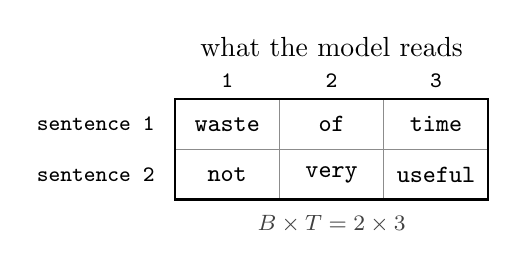
\begin{tikzpicture}[x=1.7cm]
\draw[black!45, fill=white] (0.000,0.000) rectangle (0.780,-0.640);
\node[font=\small, text=black] at (0.390,-0.320) {\texttt{waste}};
\draw[black!45, fill=white] (0.780,0.000) rectangle (1.560,-0.640);
\node[font=\small, text=black] at (1.170,-0.320) {\texttt{of}};
\draw[black!45, fill=white] (1.560,0.000) rectangle (2.340,-0.640);
\node[font=\small, text=black] at (1.950,-0.320) {\texttt{time}};
\draw[black!45, fill=white] (0.000,-0.640) rectangle (0.780,-1.279);
\node[font=\small, text=black] at (0.390,-0.959) {\texttt{not}};
\draw[black!45, fill=white] (0.780,-0.640) rectangle (1.560,-1.279);
\node[font=\small, text=black] at (1.170,-0.959) {\texttt{very}};
\draw[black!45, fill=white] (1.560,-0.640) rectangle (2.340,-1.279);
\node[font=\small, text=black] at (1.950,-0.959) {\texttt{useful}};
\draw[line width=0.9pt] (0.000,0.000) rectangle (2.340,-1.279);
\node[anchor=east, font=\footnotesize\ttfamily] at (-0.080,-0.320) {sentence 1};
\node[anchor=east, font=\footnotesize\ttfamily] at (-0.080,-0.959) {sentence 2};
\node[anchor=south, font=\footnotesize\ttfamily] at (0.390,0.020) {1};
\node[anchor=south, font=\footnotesize\ttfamily] at (1.170,0.020) {2};
\node[anchor=south, font=\footnotesize\ttfamily] at (1.950,0.020) {3};
\node[anchor=south, font=\normalsize] at (1.170,0.420) {what the model reads};
\node[anchor=north, font=\footnotesize, text=black!75] at (1.170,-1.359) {$B\times T=2\times3$};
\end{tikzpicture}
\qquad
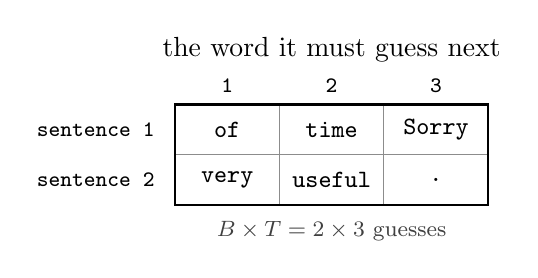
\begin{tikzpicture}[x=1.7cm]
\draw[black!45, fill=white] (0.000,0.000) rectangle (0.780,-0.640);
\node[font=\small, text=black] at (0.390,-0.320) {\texttt{of}};
\draw[black!45, fill=white] (0.780,0.000) rectangle (1.560,-0.640);
\node[font=\small, text=black] at (1.170,-0.320) {\texttt{time}};
\draw[black!45, fill=white] (1.560,0.000) rectangle (2.340,-0.640);
\node[font=\small, text=black] at (1.950,-0.320) {\texttt{Sorry}};
\draw[black!45, fill=white] (0.000,-0.640) rectangle (0.780,-1.279);
\node[font=\small, text=black] at (0.390,-0.959) {\texttt{very}};
\draw[black!45, fill=white] (0.780,-0.640) rectangle (1.560,-1.279);
\node[font=\small, text=black] at (1.170,-0.959) {\texttt{useful}};
\draw[black!45, fill=white] (1.560,-0.640) rectangle (2.340,-1.279);
\node[font=\small, text=black] at (1.950,-0.959) {\texttt{.}};
\draw[line width=0.9pt] (0.000,0.000) rectangle (2.340,-1.279);
\node[anchor=east, font=\footnotesize\ttfamily] at (-0.080,-0.320) {sentence 1};
\node[anchor=east, font=\footnotesize\ttfamily] at (-0.080,-0.959) {sentence 2};
\node[anchor=south, font=\footnotesize\ttfamily] at (0.390,0.020) {1};
\node[anchor=south, font=\footnotesize\ttfamily] at (1.170,0.020) {2};
\node[anchor=south, font=\footnotesize\ttfamily] at (1.950,0.020) {3};
\node[anchor=south, font=\normalsize] at (1.170,0.420) {the word it must guess next};
\node[anchor=north, font=\footnotesize, text=black!75] at (1.170,-1.359) {$B\times T=2\times3$ guesses};
\end{tikzpicture}
